With our parameters fully defined we can begin work on the library that applies the features we have listed.
the goal of the discovery tool itself is to provide a set of features that allow loading, matching, and manipulation
of metadata.

\subsubsection{Approach}
To begin with, we have to establish how the project itself will be handled.

We have decided to implement the tool in python - as it is a language that allows for rapid development and has
libraries heavily geared towards data manipulation such as pandas~\cite{pythonpandas}, which we will take advantage of
to provide performance efficient functionality.

Next we choose our appropriate version control - here we will be using git, and GitHub~\cite{github} for hosting our git
repository.
Using GitHub allows us to use the actions feature, which can run specific scripts depending on actions that occur within
the repository - we will be using this feature aid with our testing and deployment.

Due to the nature of the project involving handling large data files, our primary concern is avoiding loading too much
into memory, as we may run into situations where a single catalogue item's data size is larger than the available ram
for the computer.
To combat this we will rely on handling data in chunks - this means that reading, processing, and matching data must
all be capable of handling incomplete datasets, and processing sections of it instead of a single unit.

Requirements are a big part of creating usable python libraries, when there are many libraries involved in a project -
some relying on various different versions of lower level libraries, there may be clashes or mismatches.
An easy way to resolve this is to use a package management tool that can easily resolve requirements and their versions.
for this project we will be taking advantage of pdm~\cite{pythonpdm}, a lightweight python package management tool which
abstracts many more complex intricacies of python dependencies.

\subsubsection{Implementation}
In this section we will provide an overview of the decisions made when creating an implementation of the discovery
library.

To define our approach to the structure of the library, we first had to understand the desired structure of the end
product.
For example, to load a file we might expect the user to import the library, then run a snippet such as
``\textbf{discovery.load\_files(path)}''.
Following this process, we defined the resources that a user should be able to access once they have installed the
library, they are as follows:

\bigbreak
\textbf{Utilities}

- add a catalogue item

- load a local data file as metadata

- recursively load all the applicable data files starting from a path as metadata

- construct a metadata relationship between loaded catalogue items

- write generated metadata to a file

- construct a visualisation of the loaded metadata

Utilities will be included in a ``\textbf{utils}'' folder, the entrypoint script ``\textbf{discovery.py}'' will then be
the access point to each of the above given functionalities.
Users planning on taking advantage of the above functionality will be required to import the discovery class and
instantiate it, then access the methods inside of it.

\bigbreak
\textbf{metadata}

- construct a catalogue item using a specific builder with specific parameters (to create a csv file, we will use
\textbf{metadata.from\_csv})

- construct a single metadata item based on input parameters

- construct a single metadata column based on input parameters

- construct a single metadata relationship based on input parameters

In Section~\ref{sec:metadata} we have defined the format of the metadata, this Section will focus on building and
consuming it.
For the purposes of users accessing the library, we have decided to separate metadata concerns from the
``\textbf{discovery.py}'' entrypoint, this allows manipulation of metadata without having to interact with the other
features we have built.
Here we will take advantage of the python module initialisation functionality - users accessing metadata features
will do so via ``\textbf{discovery.metadata.<metadata\_utility>}''.
Additionally, we have created a set of metadata builders, which allow users to automatically build catalogue items
based on the type of data set they are using - for example, to build a catalogue item using a csv, the user can invoke
``\textbf{discovery.metadata.from\_csv(<file\_path>)}''.
These metadata builders allow us to create the more complex data loaders that we require for reading chunked data, this
means that the user does not have to be responsible for finding ways to manage their RAM usage.

\bigbreak
\textbf{Column Matching}

- expose each matching method as a class with input parameters, in the form of
``\textbf{discovery.data\_matcher.<matching\_method>(parameters)}''

- match two catalogue items with each other

Similarly to metadata, we intend to give users the option of accessing data matching without having to instantiate the
discovery class - this has led to a similar implementation.
As we have built multiple forms of data matching, we can expose each of these as a custom class that receives two pieces
of information, then return the structure that we have defined for predicting relationships.
We have also created a data matcher interface parent class, which every data matching utility must inherit - this will
help ensure type safety, and keep input parameters and output structures consistent.

For data matching, we expose a dataframe matcher utility, which consumes two catalogue items, a set of data matching
methods, and a set of weights in reference to the data matching methods.
The purpose of this setup is to allow a user to match two catalogue items based on the given matching methods, returning
a single confidence for each column intersection (modified by the weight of each matching method).

\subsubsection{Testing}
To ensure that the project maintains functionality despite changes that we make, we look towards unit tests as a metric
that can be used to define success parameters to reach.
The tool we rely on to perform this unit tests is PyTest~\cite{PyTest}.

Previously in the approach section we defined two main functionalities that easily lend themselves to unit testing -
the individual catalogue data builders, and the data matcher methods.
For our project we will ensure that at least one unit test exists for each individual object for these two
functionalities.

\begin{figure}[H]
    \centering
    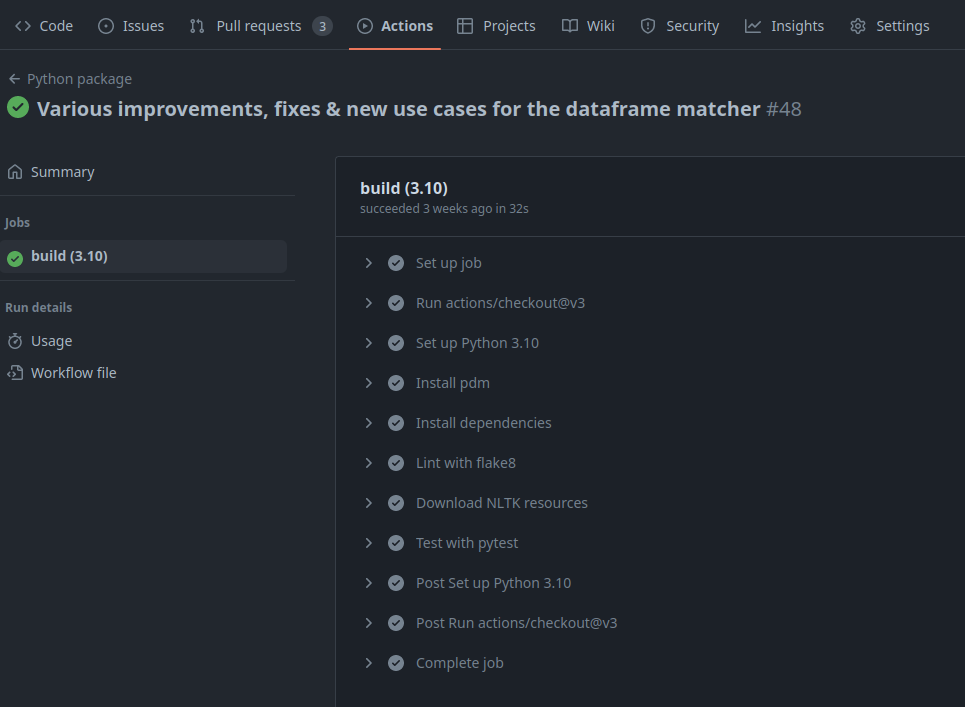
\includegraphics[width=12cm]{figures/discovery_library/test_and_lint_github_action}
    \caption{An example of a single pull request testing and linting action}
    \label{fig:discovery_unit_test}
\end{figure}

We can then further take advantage of these unit tests and the GitHub Actions feature to construct regression tests
that prevent pull requests from accidentally breaking previously working features.
To do this, we configure a GitHub action that runs pytest on our test module, and then require a pull request to have
all tests passing before allowing it to be merged.
In~\ref{fig:discovery_unit_test} we can see an example of the action running in a pull request, additionally we have
used the Flake8~\cite{Flake8} linter to ensure that code conventions have been met.

\subsubsection{Distribution}
With the tool developed, we must find a rational way to distribute the tool to potential users, and how we will provide
them access to documentation of the project functionality.

\begin{figure}[H]
    \centering
    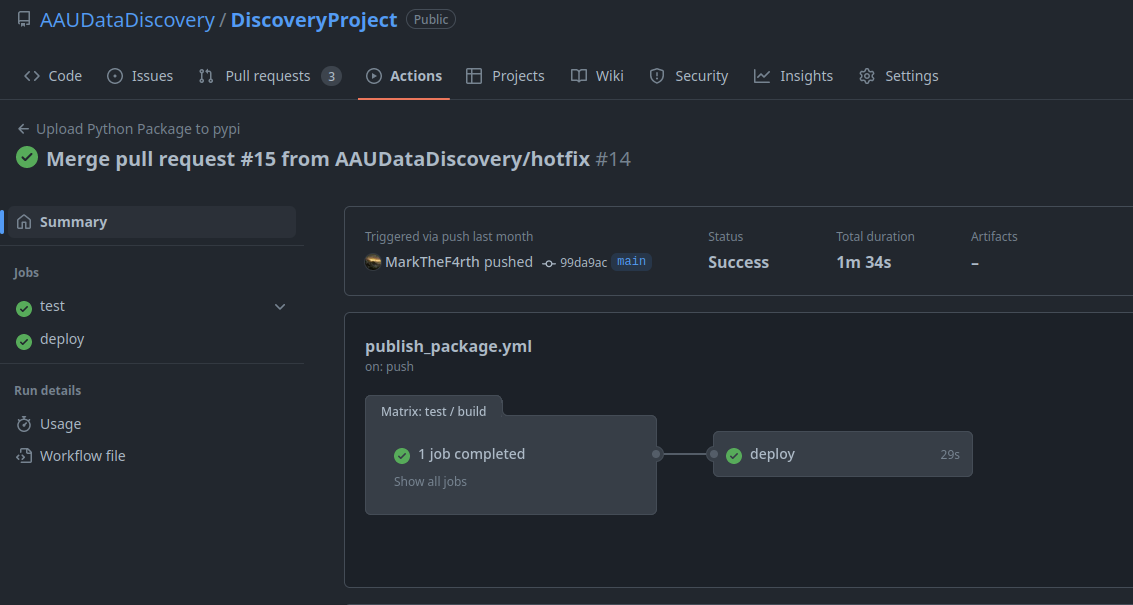
\includegraphics[width=12cm]{figures/discovery_library/github_action_test_and_deploy}
    \caption{An example of a completed pull request, running the test action and then deploying}
    \label{fig:discovery_test_and_deploy}
\end{figure}

\begin{figure}[H]
    \centering
    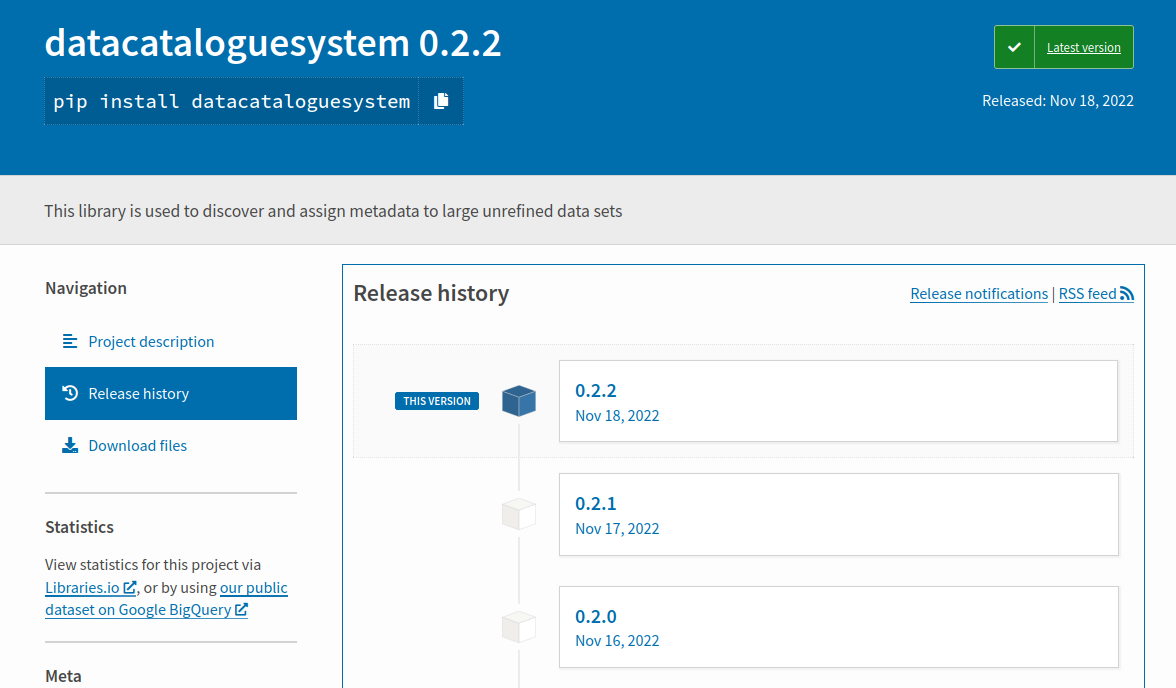
\includegraphics[width=12cm]{figures/discovery_library/pypi_catalogue_upload}
    \caption{The release history of the deployed catalogue system library}
    \label{fig:discovery_pypi_upload}
\end{figure}

Open source python libraries rely on a central public repository called pypi~\cite{PyPi} - to ensure that users have
ease of access to our project, we will similarly host the library there.
With an account created, the only real work involved in this step is to create a pipeline for uploading new releases to
the pypi repository.
For this purpose we can look back to pdm, which has an in-built publishing tool, allowing us to simply create a new
GitHub action responsible for running the \textbf{publish} command which is illustrated
in~\ref{fig:discovery_test_and_deploy}.
With all these steps complete, we can demonstrate the library being accessible on PyPi as in
figure:~\ref{fig:discovery_pypi_upload}.

Lastly, we must document the library, allowing users to have a reference guide for its usage.
For this purpose we will be using the open source documentation tool~\cite{Sphinx}, a tool which features an automatic
documentation library that allows us to build documentation based on python docstrings.
Using the auto documentation feature, we can build a static html file that lists the features of our application,
allowing not only accessible, but easily updatable documentation.
With the documentation html generated, we can use AWS to host a static website that is publicly available.

\begin{figure}[H]
    \centering
    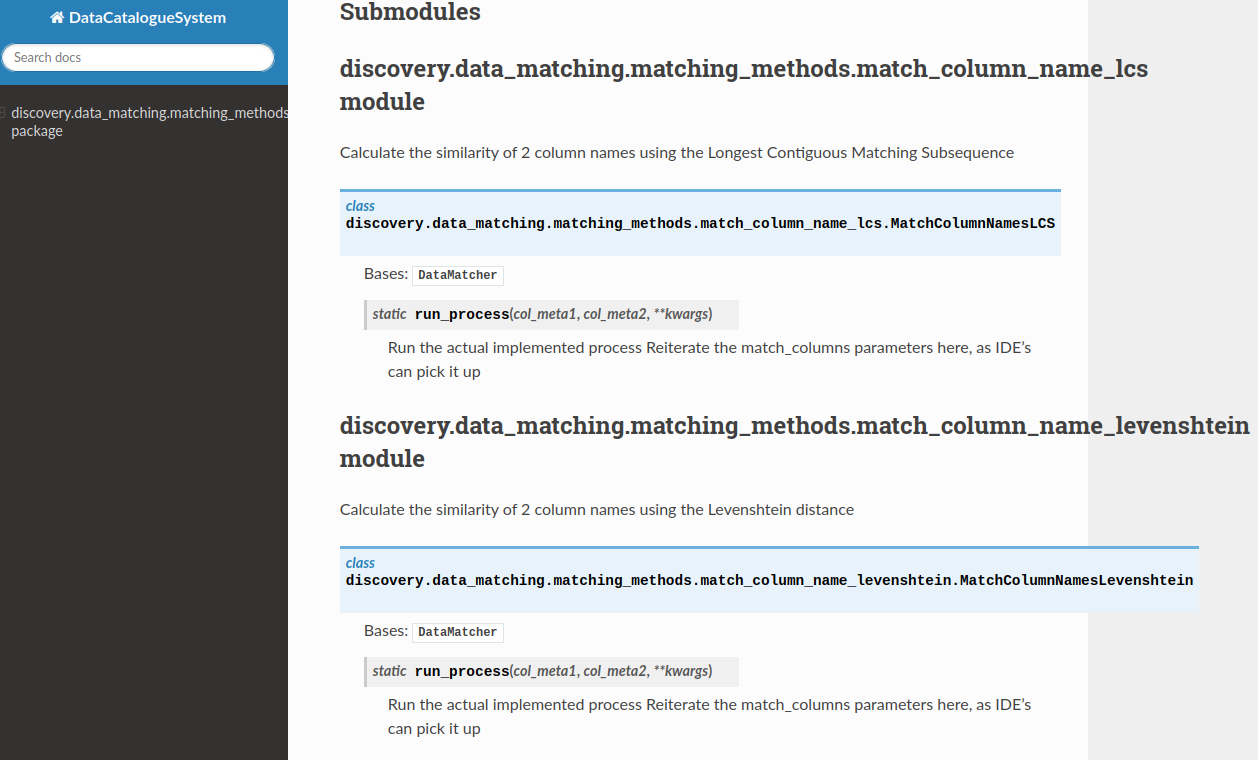
\includegraphics[width=12cm]{figures/discovery_library/discovery_client_documentation}
    \caption{A snippet of the data matching methods within the automatically generated documentation}
    \label{fig:discovery_client_documentation}
\end{figure}

We can see the results of the automatic documentation in~figure~\ref{fig:discovery_client_documentation}, unfortunately
the presentation does require some tweaking before being presentable to end users, however this is a good example of how
easy it is to set up something useful with minimal effort.

\subsubsection{Reflections}
From the beginning, we built the library with future additions in mind, we believe that the structure we built has
managed to adequately achieve a robustness that allows for more specialised features to be created in the future.
Creating new methods for data matching, data loading, or utilities that perform various analytics - all of these can be
easily built on top of the existing structure without significant edits.
